\documentclass[../main.tex]{subfiles}
\begin{document}
\subsection*{Vector Operation}
There are four vector operation: Addition,  Multiplication by a scalar, Dot product, and Cross Product.
(i) Addition of two vectors. Addition is commutative and associative
\begin{align*}
    \A+\B&=\B+\A\\
    (\mathbf{A }+ \B) +\mathbf{ C}& = \mathbf{A }+ (\B + \C).
\end{align*}

(ii) Multiplication by a scalar. Scalar multiplication is distributive.
\begin{align*}
    a(\A + \mathbf{\B}) = a\A + a\B
\end{align*}

(iii) Dot product of two vectors. The dot product of two vectors is defined 
\begin{align*}
    \A \cdot \B \equiv AB \cos \theta
\end{align*}
where $\theta$ is the angle they form. Note that dot product is commutative and distributive.
\begin{align*}
    \A \cdot \B &= \B \cdot \A\\
    \A \cdot (\B + \C) &= \A \cdot \B + \A \cdot \C
\end{align*}

(iv) Cross product of two vectors. The cross product of two vectors is defined by
\begin{align*}
    \A \times \B \equiv AB \sin \theta\;\mathbf{ \hat{n}}
\end{align*}
where $\mathbf{\hat{n}}$ is a unit vector pointing perpendicular to the plane of $\A$ and $\B$.  The cross product is distributive, but not commutative.
\begin{align*}
    \A \times (\B + \C) &= (\A \times \B) + (\A \times \C)\\
    (\B \times \A) &= -(\A \times \B)
\end{align*}

Few rule for manipulating vector. (i): To add vectors, add like components
\begin{align*}
    \A + \B=(A_x + B_x )\mathbf{\hat{x}} + (A_y + B_y )\mathbf{\hat{y}} + (A_z + B_z )\mathbf{\hat{z}}
\end{align*}
(ii): To multiply by a scalar, multiply each component.
\begin{align*}
    a\A = (a A_x )\mathbf{\hat{x}}+ (a A_y )\mathbf{\hat{y}} + (a A_z )\mathbf{\hat{z}}
\end{align*}
Rule (iii): To calculate the dot product, multiply like components, and add.
\begin{align*}
    \A \cdot \B &= A_xB_x +A_yB_y+ A_zB_z \\
\end{align*}

Rule (iv): To calculate the cross product, form the determinant whose first row is unit vector, whose second row is A (in component form), and whose third row is B.
\begin{align*}
    \A\times \B&=
    \begin{vmatrix}
        \mathbf{\hat{x}}&\mathbf{\hat{y}}&\mathbf{\hat{z}}\\
        A_x&A_y&A_z\\
        B_x&B_y&B_z
    \end{vmatrix}
\end{align*}

\subsection*{Triple Product}

(i) Scalar triple product. 
\begin{align*}
    \A \cdot (\B \times \C) = B \cdot (\C \times A) = C \cdot (\A \times B)
\end{align*}
They are cyclic and in component form\begin{align*}
    \A \cdot (\B \times \C)&=\begin{vmatrix}
        A_x&A_y&A_z\\
        B_x&B_y&B_z\\
        C_x&C_y&C_z
    \end{vmatrix}
\end{align*}

(ii) Vector triple product.
\begin{equation*}
    \A \times (\B \times \C) = \B(\A \cdot \C) - \C(\A \cdot \B).
\end{equation*}
The product is linear combination of vector in parentheses.

\subsection*{Separation Vector}
Separation vector defined as vector from the source point $\bar{r'}$ to the field point $\bar{r}$
\begin{equation*}
    \rcurs \equiv \mathbf{\bar{r} }- \mathbf{\bar{r'}}.
\end{equation*}

\begin{figure}[b]
    \centering
    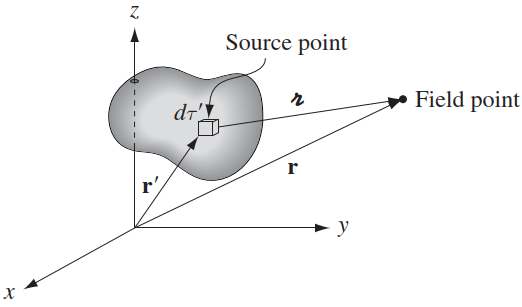
\includegraphics[width=0.65\textwidth]{SepVec.png}
    \caption*{Figure: Separation vector}
\end{figure}

\subsection*{Del Operator}
Vector operator defined as follows.
\begin{equation*}
    \nabla = \mathbf{\hat{x}}\frac{\partial}{\partial x}+\mathbf{\hat{y}}\frac{\partial}{\partial y}+\mathbf{\hat{z}}\frac{\partial}{\partial z}
\end{equation*}

\subsection*{Operation Involving Del Operator}
There are three ways the operator $\nabla$ can act:
\begin{enumerate}
    \item On a scalar function $T$ : $\nabla T$ (the gradient); 
    \item On a vector function $\mathbf{v}$, via the dot product: $\nabla \cdot \mathbf{v}$ (the divergence); 
    \item On a vector function $\mathbf{v}$, via the cross product: $\nabla \times \mathbf{v}$ (the curl).
\end{enumerate}

Gradient of scalar function $T(x,y,z)$  
\begin{equation*}
    \nabla T = \mathbf{\hat{x}}\frac{\partial T}{\partial x}+\mathbf{\hat{y}}\frac{\partial T}{\partial y}+\mathbf{\hat{z}}\frac{\partial T}{\partial z}
\end{equation*}
can be used to define partial derivative of $T$ 
\begin{align*}
    dT&= \bigg(  \mathbf{\hat{x}}\frac{\partial T}{\partial x}+ \mathbf{\hat{y}}\frac{\partial T}{\partial y}+ \mathbf{\hat{z}}\frac{\partial T}{\partial z} \bigg)\cdot (dx\;  \mathbf{\hat{x}}+dy\; \mathbf{\hat{y}}+dz\; \mathbf{\hat{z}})\\
    &=\nabla T \cdot \mathbf{\hat{u}}
\end{align*}
Note that $\nabla T$ is a vector quantity, with three components. The gradient $\nabla T$ points in the direction of maximum increase of the function $T$. Moreover, The magnitude $\nabla T$ gives the slope (rate of increase) along this maximal direction.

Divergence of vector function \textbf{V} is
\begin{align*}
    \nabla \cdot  \mathbf{v}= \frac{\partial v_x}{\partial x}+\frac{\partial v_y}{\partial y}+\frac{\partial v_z}{\partial z}
\end{align*}
which is a scalar. Divergence is a measure of how much the vector V spreads out (diverges) from the point in question.

Curl of vector function \textbf{V} is
\begin{equation*}
    \nabla \times  \mathbf{v}=
    \begin{vmatrix}
         \mathbf{\hat{x}}& \mathbf{\hat{y}}& \mathbf{\hat{z}}\\
        \dfrac{\partial }{\partial x}&\dfrac{\partial}{\partial y}&\dfrac{\partial }{\partial z}\\
        V_x&V_y&V_z
    \end{vmatrix} 
\end{equation*}
The name curl is also well-chosen, for $\nabla \times  \mathbf{v}$ is a measure of how much the vector \textbf{v} swirls around the point in question. 

\subsection*{Product Rule}
There are two ways to construct a scalar as the product of two functions
\begin{align*}
    fg\quad&\text{(product of two scalar functions)}\\
    \A\cdot \B\quad&\text{(dot product of two vector functions)}
\end{align*}
and two ways to make a vector
\begin{align*}
    f\A\quad&\text{(scalar times vector)}\\
    \A\times \B\quad&\text{(cross product of two vectors)}
\end{align*}
Accordingly, there are six product rule, two for gradients
\begin{equation*}
    \nabla ( f g) = f \nabla g + g\nabla f
\end{equation*}
\begin{equation*}
    \nabla(\A \cdot \B) = \A \times (\nabla \times  \B) + \B \times  (\nabla \times  \A) + (\A \cdot \nabla)\B + (\B \cdot \nabla)\A
\end{equation*}
two for divergences
\begin{equation*}
    \nabla ( f \A) = f (\nabla \cdot \A) + \A\cdot(\nabla f)
\end{equation*}
\begin{equation*}
    \nabla\cdot (\A \times \B) = \B\cdot (\nabla \times  \A)-\A\cdot (\nabla \times \B)
\end{equation*}
and two for curls
\begin{equation*}
    \nabla \times ( f \A) = f (\nabla \times \A) - \A \times (\nabla f )
\end{equation*}
\begin{equation*}
    \nabla \times (\A \times \B) = (\B \cdot \nabla)\A - (\A \cdot \nabla)\B + \A(\nabla \cdot \B) - \B(\nabla \cdot \A)
\end{equation*}

\subsection*{Second Derivative}

(1) Divergence of gradient: $\nabla \cdot (\nabla T)$. 
Called Laplacian of T. Notice that the Laplacian of a scalar T is a scalar. 
\begin{equation*}
    \nabla^2 T=\frac{\partial^2T}{\partial x}+\frac{\partial^2T}{\partial y}+\frac{\partial^2T}{\partial z}
\end{equation*}
Occasionally, we shall speak of the Laplacian of a vector, $\nabla ^2  \mathbf{v}$. By this we mean a vector quantity whose $x$-component is the Laplacian of $V_x$, and so on:
\begin{equation*}
    \nabla^2 \mathbf{v} \equiv (\nabla^2 V_x ) \mathbf{\hat{x}} + (\nabla^2 V_y)\hat{y} + (\nabla^2 V_z ) \mathbf{\hat{z}}
\end{equation*}

(2) The curl of a gradient: $\nabla \times (\nabla T)$. Always zero.
\begin{equation*}
    \nabla \cdot (\nabla T)=0
\end{equation*}

(3) Gradient of divergence: $\nabla  (\nabla \cdot  \mathbf{v})$. 
$\nabla  (\nabla \cdot  \mathbf{v})$ is not the same as the Laplacian of a vector.
\begin{equation*}
    \nabla  (\nabla \cdot  \mathbf{v}) \neq \nabla^2  \mathbf{v} = (\nabla \cdot \nabla)  \mathbf{v} 
\end{equation*}

(4) The divergence of a curl: $\nabla  \cdot (\nabla \times  \mathbf{v})$. Always zero.
\begin{equation*}
    \nabla \cdot (\nabla \times  \mathbf{v})=0
\end{equation*}

(5) Curl of curl:$\nabla \times (\nabla \times  \mathbf{v})$. From the definition of $\nabla$, 
\begin{equation*}
    \nabla \times (\nabla \times  \mathbf{v})=\nabla (\nabla \cdot  \mathbf{v})-\nabla^2 \mathbf{v}
\end{equation*}

\subsection*{Fundamental Theorem of Calculus}
The fundamental theorem of calculus says the integral of a derivative over some region is given by the value of the function at the end points (boundaries). 
\begin{equation*}
    \int_{a}^{b} \frac{df}{dx}\;dx=f(b)-f(a)
\end{equation*}

\subsubsection*{Gradient.} The fundamental theorem for gradients; like the “ordinary” fundamental theorem, it says that the integral (line integral) of a derivative (gradient) is given by the value of the function at the boundaries (a and b).
\begin{equation*}
    \int_{a}^{b}(\nabla T)\cdot d\mathbf{l}=T(\mathbf{b})-T(\mathbf{a})
\end{equation*}

\emph{Corollary 1:} $ \int_{a}^{b}(\nabla T)\cdot d\mathbf{l}$ is independent of the path.

\emph{Corollary 2:} $\oint (\nabla T)\cdot d\mathbf{l}=0 $ since the beginning and end points are identical.

\subsubsection*{Divergences}.
Like the other “fundamental theorems,” it says that the integral of a derivative (divergence) over a region (volume V) is equal to the value of the function at the boundary (surface S).
\begin{equation*}
    \int_{V}(\nabla \cdot \mathbf{v})\;d\tau=\oint_{S}\mathbf{v}\cdot d\mathbf{a}
\end{equation*}

If v represents the flow of an incompressible fluid, then the flux of $\mathbf{v}$ is the total amount of fluid passing out through the surface, per unit time.  There are two ways we could determine how much is being produced: (a) we could count up all the faucets, recording how much each puts out, or (b) we could go around the boundary, measuring the flow at each point, and add it all up. Alternatively,
\begin{equation*}
    \int (\text{faucets within the volume})=\oint (\text{flow out through the surface})
\end{equation*}

\subsubsection*{Curl.} As always, the integral of a derivative (curl) over a region (patch of surface, $S$) is equal to the value of the function at the boundary (perimeter of the patch, $P$). Now, the integral of the curl over some surface (flux of the curl) represents the “total amount of swirl,” and we can determine that just as well by going around the edge and finding how much the flow is following the boundary.
\begin{equation*}
    \int_{S}(\nabla \times \mathbf{v})\cdot d\mathbf{a}=\oint_{P}\mathbf{v}\cdot d\mathbf{l}
\end{equation*}

\emph{Corollary 1.} $\int (\nabla \times \mathbf{v})\cdot d\mathbf{a}$ depends only on the boundary line. It doesn't matter which way you go as long as you are consistent. For a closed surface (divergence theorem), $d\mathbf{a}$ points in the direction of the outward normal; but for an open surface is given by the right-hand rule: if your fingers point in the direction of the line integral, then your thumb fixes the direction of $d\mathbf{a}$.

Corollary 2. $\oint (\nabla \times \mathbf{v})\cdot d\mathbf{a}=0$ for any closed surface, since the boundary line, like the mouth of a balloon, shrinks down to a point.

\subsection*{Integration by Parts}
It applies to the situation in which you are called upon to integrate the product of one function $( f )$ and the derivative of another $(g)$; it says you can transfer the derivative from $g$ to $f$, at the cost of a minus sign and a boundary term.
\begin{equation*}
    \int_{a}^{b} f\bigg(\frac{dg}{dx}\bigg)\;dx=-\int_{a}^{b} g\bigg(\frac{df}{dx}\bigg)\;dx+ fg \bigg\lvert_{a}^{b}
\end{equation*}

\subsection*{Curvilinear Coordinates}
I shall use arbitrary (orthogonal) curvilinear coordinates ($u, v, w$), developing formulas for the gradient, divergence, curl, and Laplacian in any such system. Infinitesimal displacement vector can be written
\begin{equation*}
    d\mathbf{l}=f\;d u \;\mathbf{\hat{u}} +g \;d v \;\mathbf{\hat{v}}+h \;d w \;\mathbf{\hat{w}}
\end{equation*}
where $f$, $g$, and $h$ are functions of position characteristic of the particular coordinate system. While infinitesimal volume is
\begin{equation*}
    d\tau=fgh\; du \;dv \;dw
\end{equation*}
Use table \ref{T1} for references.

\begin{table}
    \centering
    \caption{Table}
    \begin{tabular}{c c c c c c c } 
        \toprule
        System&$u$&$v$&$w$&$f$&$g$&$h$\\
        \midrule
        Cartesian&$x$&$y$&$z$&1&1&1\\
        Spherical&$r$&$\theta$&$\phi$&1&$r$&$r$ $\sin \theta$\\
        Cylindrical&$s$&$\phi$&$z$&1&$s$&$1$\\
        \bottomrule
    \end{tabular}
    \label{T1}
\end{table}

\subsubsection*{Gradient.} The gradient of t is
\begin{equation*}
    \nabla \mathbf{t} \equiv \frac{1}{f}\frac{\partial t}{\partial u}\mathbf{\hat{u}}+ \frac{1}{g}\frac{\partial t}{\partial v}\mathbf{\hat{v}}+ \frac{1}{h}\frac{\partial t}{\partial w}\mathbf{\hat{w}}
\end{equation*}

\subsubsection*{Divergence.} The divergence of $\A$ in curvilinear coordinates:
\begin{equation*}
    \nabla \cdot \A\equiv \frac{1}{fgh} \biggl[ \frac{\partial}{\partial u} (ghA_u)+ \frac{\partial}{\partial v} (fh A_v)+\frac{\partial}{\partial w} (fg A_w)\biggr]
\end{equation*}

\subsubsection*{Curl.} 
\begin{multline*}
    \nabla \times \A\equiv \frac{1}{gh} \biggl[\frac{\partial}{\partial v} (hA_w) -\frac{\partial}{\partial w } (g A_{v}) \biggr]\mathbf{\hat{u}}
    +\frac{1}{fh} \biggl[\frac{\partial}{\partial w} (f A_{u}) -\frac{\partial}{\partial u } (h A_{w}) \biggr]\mathbf{\hat{v}}\\
    +\frac{1}{fg} \biggl[\frac{\partial}{\partial u} (g A_{v}) -\frac{\partial}{\partial v } (f A_{u}) \biggr]\mathbf{\hat{w}}
\end{multline*}

\subsubsection*{Laplacian.} 
\begin{equation*}
    \nabla^2t\equiv \frac{1}{fgh}\biggl[\frac{\partial}{\partial u}\Biggl(\frac{gh}{f}\frac{\partial t}{\partial u}\Biggr)+ \frac{\partial}{\partial v}\Biggl(\frac{fh}{g}\frac{\partial t}{\partial v} \Biggr)+ \frac{\partial}{\partial w}\Biggl(\frac{fg}{h}\frac{\partial t}{\partial w}\Biggr)\biggr]
\end{equation*}

\subsubsection*{Spherical.}
\begin{align*}
   & \begin{cases}
        x &= r \sin \theta \cos \phi\\
        y &= r \sin \theta \sin \phi\\
        z & = r \cos \theta
    \end{cases}&&
    \begin{cases}
        \mathbf{\hat{x}} = \sin \theta \cos \phi \;\mathbf{\hat{r}} + \cos \theta \cos \phi \;\boldsymbol{\hat{\theta}} - \sin \phi \;\boldsymbol{\hat{\phi}}\\
        \mathbf{\hat{y}} = \sin \theta \sin \phi \;\mathbf{\hat{r}} + \cos \theta \sin \phi \;\boldsymbol{\hat{\theta}} + \cos \phi\;\boldsymbol{\hat{\phi}}\\
        \mathbf{\hat{z}} = \cos \theta\;\mathbf{\hat{r}} - \sin \theta \;\boldsymbol{\hat{\theta}}
    \end{cases}\\
   &
   \begin{cases}
        r &= \sqrt{x^2 + y^2 + z^2}\\
        \theta &=\arctan \sqrt{x^2 + y^2}/z\\
        \phi & = \arctan y/z
    \end{cases}&&
    \begin{cases} 
        \mathbf{\hat{r}} = \sin \theta \cos \phi \;\mathbf{\hat{x}} + \sin \theta \sin \phi \;\boldsymbol{\hat{y}} + \cos \theta \;\boldsymbol{\hat{z}}\\
        \boldsymbol{\hat{\theta}} = \cos \theta \cos \phi \;\mathbf{\hat{x}} + \cos \theta \sin \phi \;\boldsymbol{\hat{y}} - \sin \theta\;\boldsymbol{\hat{z}}\\
        \boldsymbol{\hat{\phi}} = -\sin \phi\;\mathbf{\hat{x}} + \cos \phi \;\boldsymbol{\hat{y}}
    \end{cases}
\end{align*}

\subsubsection*{Cylindrical.}
\begin{align*}
   & \begin{cases}
        x &= s \cos \phi \\
        y &= s \sin \phi \\
        z & =z
    \end{cases}&&
    \begin{cases}
        \mathbf{\hat{x}} =  \cos \phi \;\mathbf{\hat{s}}-  \sin \phi \;\boldsymbol{\hat{\phi}} \\
        \mathbf{\hat{y}} =  \sin \phi \;\mathbf{\hat{s}} + \cos \phi \;\boldsymbol{\hat{\phi}} \\
        \mathbf{\hat{z}} = \mathbf{\hat{z}} 
    \end{cases}\\
   &\begin{cases}
        s &= \sqrt{x^2 + y^2 }\\
        \phi &=\arctan y/z\\
        z & = z
    \end{cases}&&
    \begin{cases} 
        \mathbf{\hat{s}} =  \cos \phi \;\mathbf{\hat{x}} +  \sin \phi \;\boldsymbol{\hat{y}}\\
        \boldsymbol{\hat{\phi}} = -\sin  \phi \;\mathbf{\hat{x}} + \cos \phi \;\boldsymbol{\hat{y}} \\
        \boldsymbol{\hat{z}} = \boldsymbol{\hat{z}}
    \end{cases}
\end{align*}

\begin{figure*}
    \centering
    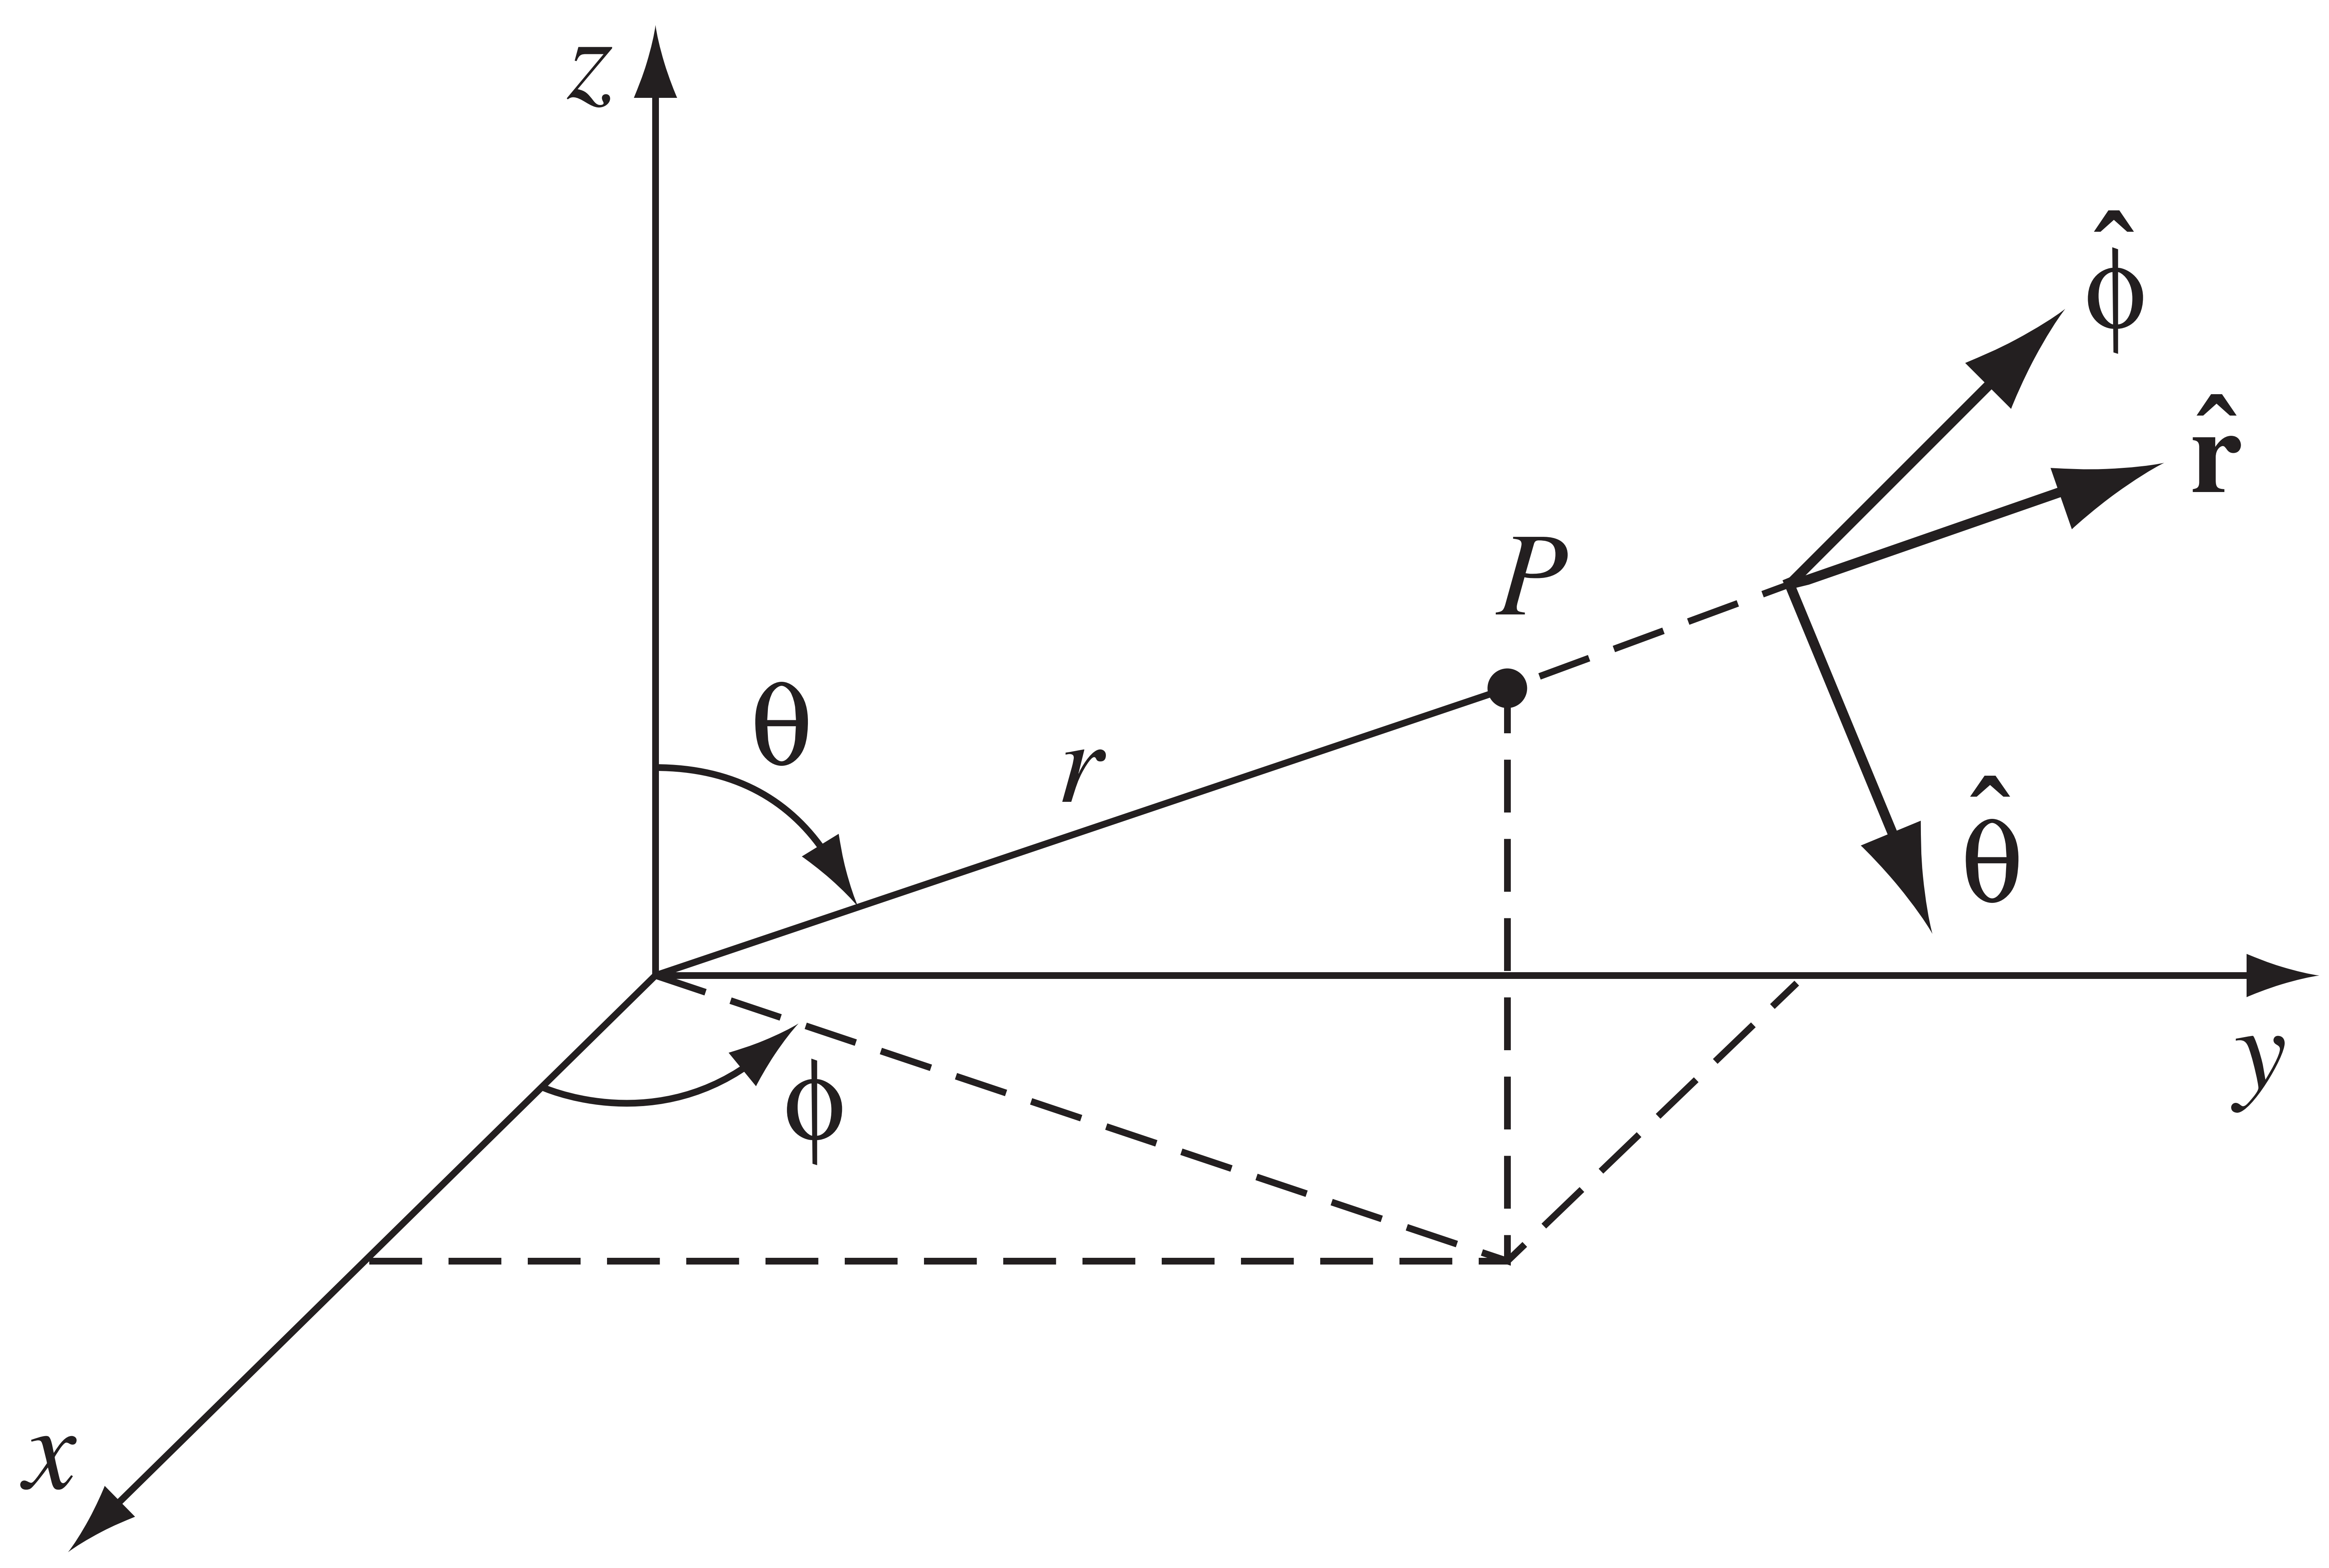
\includegraphics[width=0.4\textwidth]{Spherical.png}
    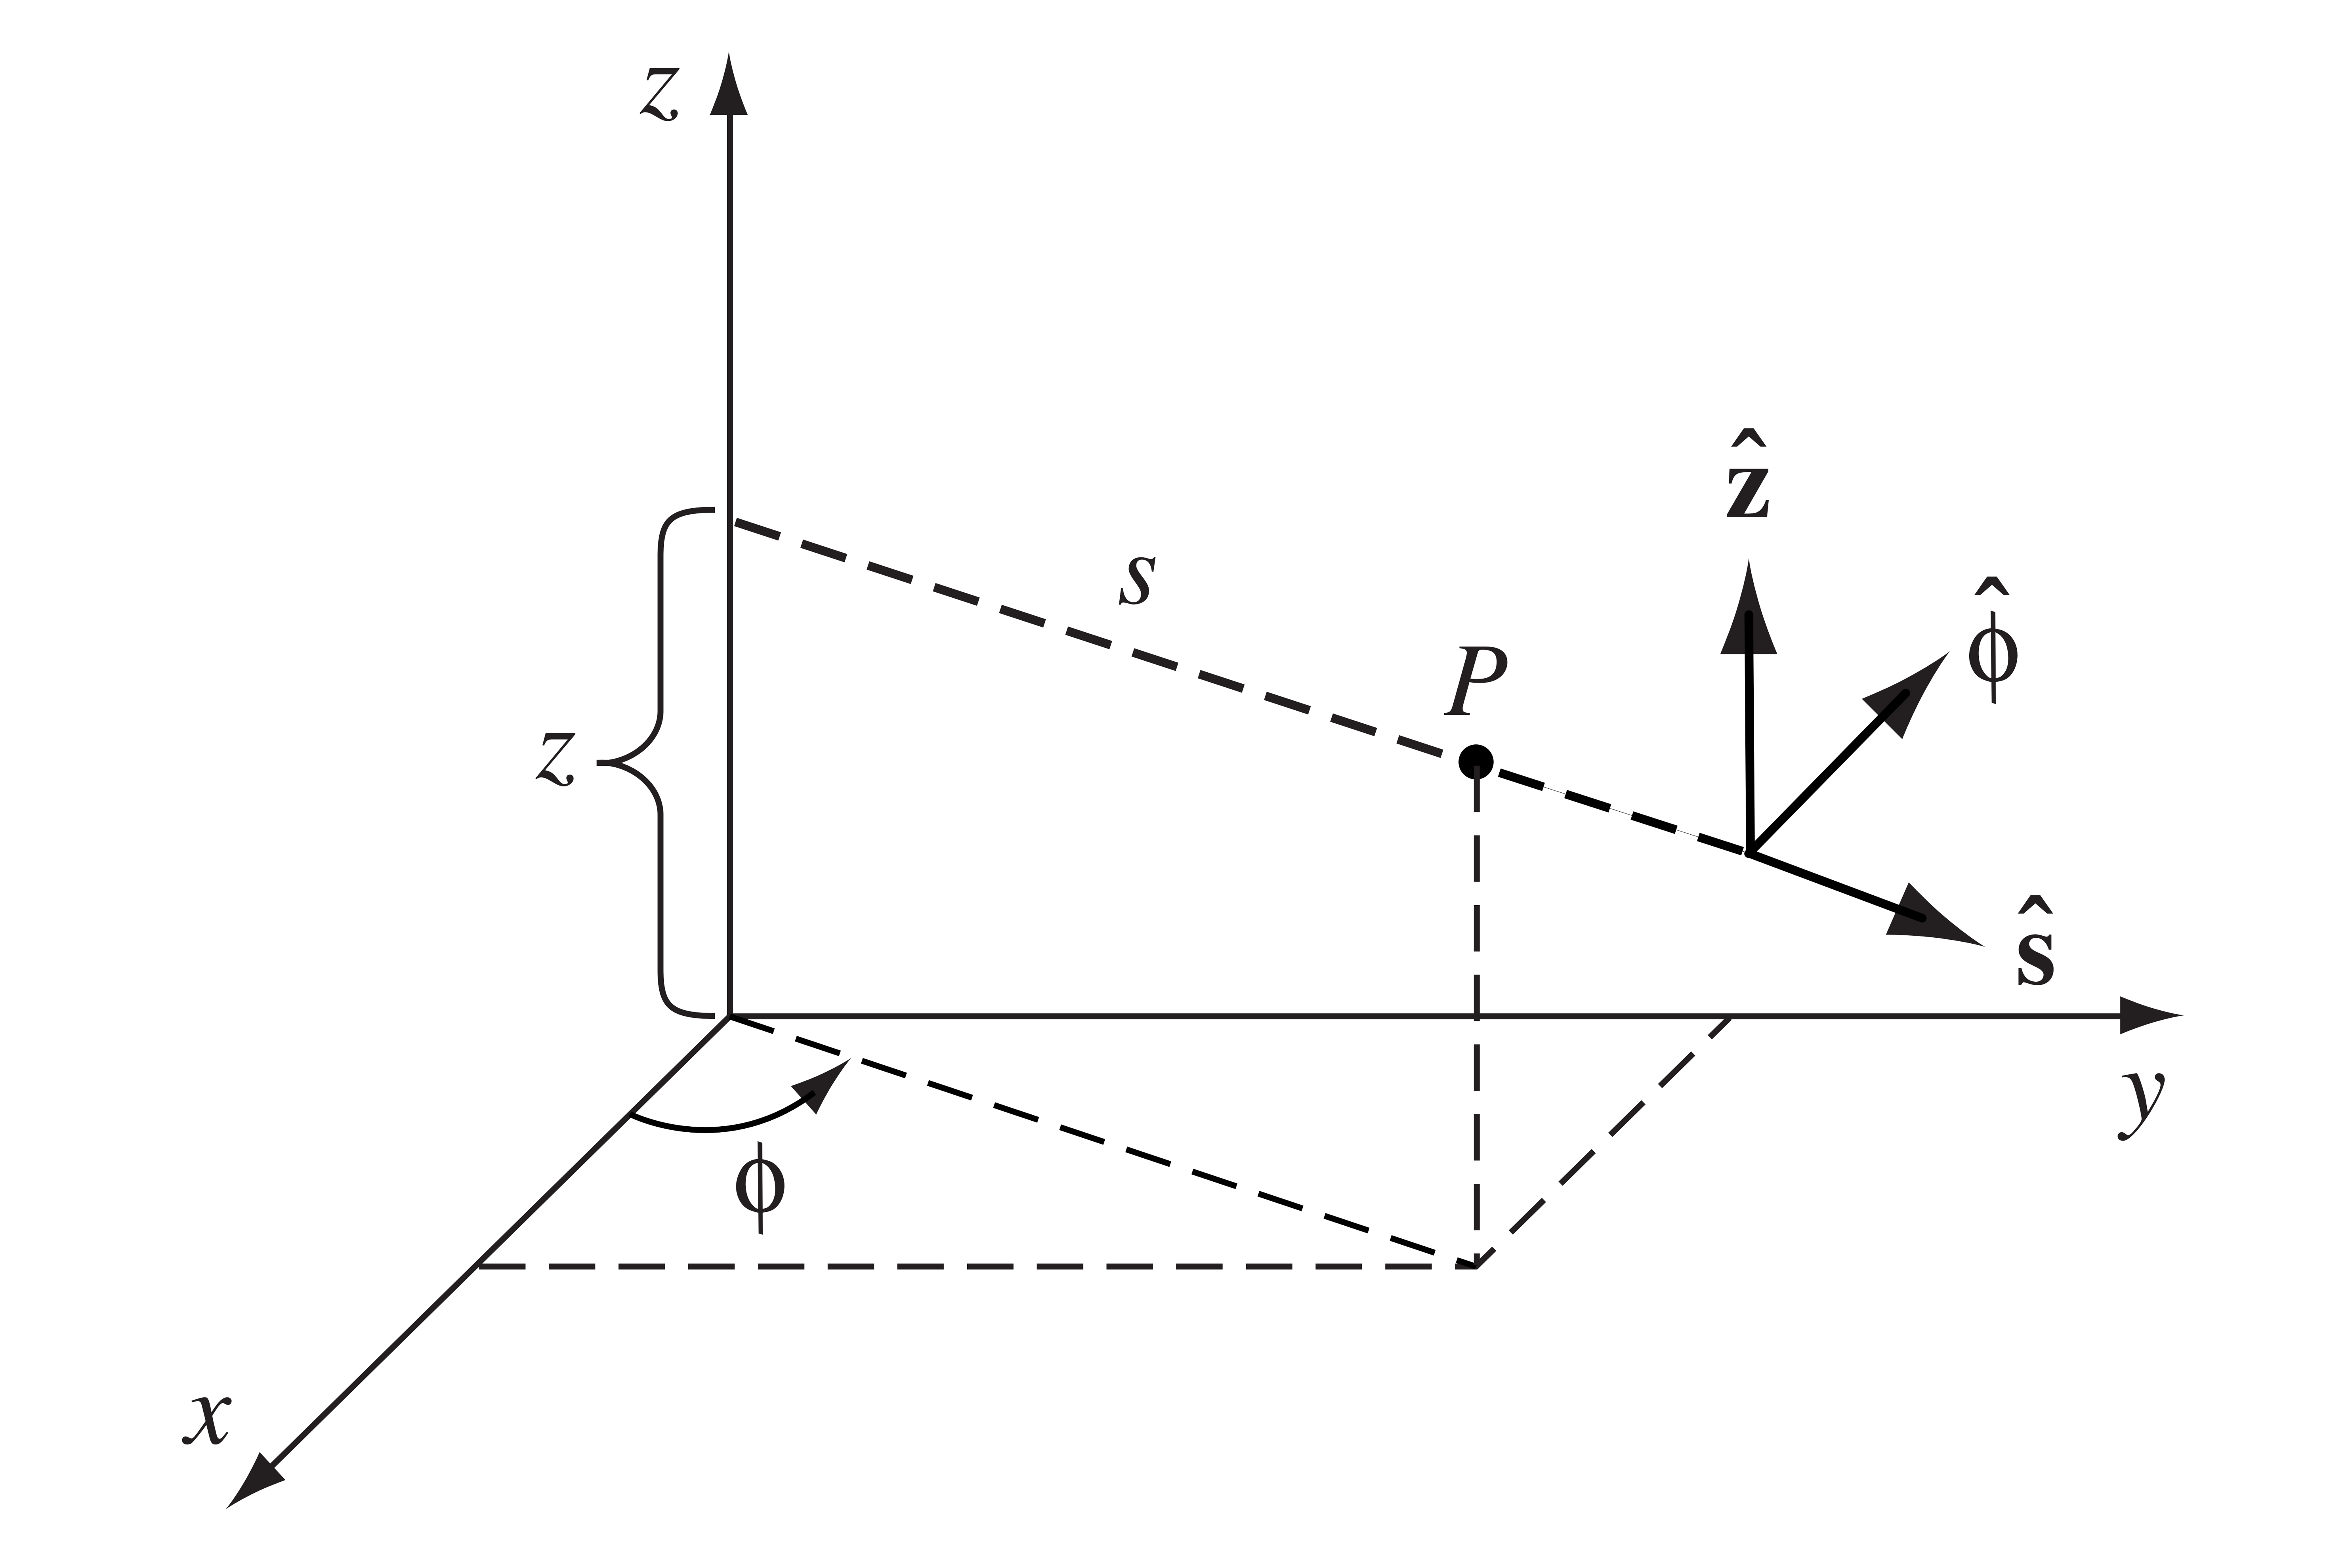
\includegraphics[width=0.4\textwidth]{Cyl.png}
    \caption*{Spherical Coordinates and Cylindrical Coordinates}
\end{figure*}

\subsection*{Dirac Delta}
The one-dimensional Dirac delta function, $\delta(x)$, can be pictured as an infinitely high, infinitesimally narrow “spike,” with area 1. That is to say
\begin{equation*}
    \delta (x-a)=\begin{cases}
        0,\quad  x\neq a\\
        \infty,\quad  x=a
    \end{cases}
\end{equation*}
with
\begin{equation*}
    \int_{-\infty}^{\infty} \delta (x-a)\;dx =1
\end{equation*}
It follows that
\begin{equation*}
    f(x)\delta(x-a)=f(a)\delta(x-a)
\end{equation*}
Since the product is zero anyway except at $x = a$, we may as well replace $f (x)$ by the value it assumes at the origin. In particular
\begin{equation*}
    \int_{-\infty}^{\infty}f(x)\delta(x-a)\;dx=f(a)
\end{equation*}
It's best to think of the delta function as something that is always intended for use under an integral sign. In particular, two expressions involving delta functions (say, $D_1(x)$ and $D_2(x)$) are considered equal if
\begin{equation*}
    \int_{-\infty}^{\infty}f(x)D_1(x)\;dx=\int_{-\infty}^{\infty}f(x)D_2(x)\;dx
\end{equation*}

It is easy to generalize the delta function to three dimensions
\begin{equation*}
    \delta^3(\textbf{r})=\delta (x)\delta (y)\delta(z)
\end{equation*}
with $\textbf{r} \equiv x \hat{x} + y\hat{y}+ z \hat{z}$, and it's integral
\begin{equation*}
    \int_{\text{all space}}\delta^3({\textbf{r}})=\int_{-\infty}^{\infty}\int_{-\infty}^{\infty}\int_{-\infty}^{\infty}\delta(x)\delta(y)\delta(z)\;dxdydz=1
\end{equation*}
Generalizing Delta function, we get
\begin{equation*}
    \int_{\text{all space}}f(\textbf{r})\delta^3({\textbf{r-a}})\;d\tau=f(\textbf{a})
\end{equation*}

Few Dirac delta function
\begin{align*}
    \nabla \cdot \biggl( \frac{\mathbf{\hat{\brcurs}}}{\rcurs ^2}\biggr)&=4\pi \delta^3(\brcurs)\\
    \nabla \biggl( \frac{1}{\rcurs}\biggr)&=-\frac{\mathbf{\hat{\brcurs}}}{\rcurs ^2}\\
    \nabla^2 \frac{1}{\rcurs}&=-4\pi \delta^3(\brcurs)
\end{align*} 

\subsubsection*{Fourier Transform of a $\boldsymbol{\delta}$ function.} Using the definition of a Fourier transform, we write
\begin{equation*}
    g(\alpha)=\frac{1}{2\pi}\int_{-\infty}^{\infty}\delta(x-a)e^{-i\alpha x}\;dx =\frac{1}{2\pi} e^{-i\alpha x}
\end{equation*}
and its inverse transform
\begin{equation*}
    \delta(x-a)=\int_{-\infty}^{\infty}g(\alpha)e^{i\alpha x}\;d\alpha=\frac{1}{2\pi} \int_{-\infty}^{\infty} e^{i\alpha (x-a)}\;d\alpha
\end{equation*}
The integral however does not converge. If we replace the limits by $-n, n$, we obtain a set of functions  which are increasingly peaked around $x = a$ as $n$ increases, but all have area 1.

\subsubsection*{Derivative of a $\boldsymbol{\delta}$ function.} Using repeated integrations by parts gives 
\begin{equation*}
    \int_{-\infty}^{\infty}\phi(x)\delta^{(n)}(x-a)\;dx=(-1)^n\phi^{(n)}(a)
\end{equation*}

\subsubsection*{Few formulas involving $\boldsymbol{\delta}$ function.} For step function
\begin{align*}
    u(x-a)&=\begin{cases}
        1,x>a\\
        0,x<a\\
    \end{cases}\\
    u'(x-a)&=\delta(x-a)
\end{align*}
It is easy to see how the derivative of step function is equal to delta function.

\subsection*{Helmholtz Theorem}
Suppose we are told that the divergence of a vector function F(r) is a specified
scalar function D(r):
\begin{equation*}
    \nabla \cdot \mathbf{F}=D
\end{equation*}
and the curl of F(r) is a specified vector function C(r):
\begin{equation*}
    \nabla \times \mathbf{F}=\C
\end{equation*}
For consistency, C must be divergenceless $\nabla \cdot \C=0$. 
Helmholtz theorem state if the divergence D(r) and the curl C(r) 
of a vector function F(r) are specified, 
and if they both go to zero faster than $1/r^2$ as $ r \rightarrow \infty$
and if F(r)
goes to zero as $ r \rightarrow \infty$, 
then F is given uniquely by
\begin{equation*}
    \mathbf{F} =-\nabla U+\nabla \times \mathbf{W}
\end{equation*}

\subsection*{Potential Theorem}
\subsubsection*{Curl-less (or “irrotational”) fields.} 
The following conditions are equivalent
(that is, F satisfies one if and only if it satisfies all the others):
\begin{itemize}
    \item $\nabla \times \mathbf{F}=0$ everywhere.
    \item  $\int_{a}^{b}\mathbf{F}\cdot\;d\mathbf{l}$ is independent of path, for any given end points.
    \item $\oint\mathbf{F} \cdot\;d\mathbf{l}=0$ for any closed loop.
    \item \textbf{F} is the gradient of some scalar function: $F =- \nabla V$ .
\end{itemize}

\subsubsection*{Divergence-less (or “solenoidal”) fields.} 
The following conditions are equivalent:
\begin{itemize}
    \item $\nabla \cdot \mathbf{F}=0$ everywhere.
    \item  $\int\mathbf{F}\cdot\;d\mathbf{a}$ is independent of surface, for any given boundary line.
    \item $\oint\mathbf{F} \cdot\;d\mathbf{a}=0$ for any closed surface.
    \item \textbf{F} is the curl  of some scalar function: $\mathbf{F} =- \nabla \A$.
\end{itemize}
\end{document}  

